\esSezione{Rete di interconnessione 16:4}\label{sec:esercizio1-2}

\begin{traccia}
Utilizzando il componente sviluppato al punto precedente, progettare, implementare in VHDL e testare mediante simulazione una rete di interconnessione a 16 sorgenti e 4 destinazioni.
\end{traccia}

\progetto

La rete comprende due componenti: il multiplexer \texttt{mux\_16\_1}, che seleziona uno dei 16 ingressi mediante il segnale \texttt{s\_i} a 4 bit, e il demultiplexer \texttt{demux\_1\_4}, che ripropone il bit selezionato su una delle 4 uscite in base al segnale \texttt{s\_o} a 2 bit. Il bit intermedio transita nel segnale interno \texttt{q}, di un solo bit. Il multiplexer 16:1 è già stato presentato nell'esercizio~1.1, insieme al multiplexer 4:1 su cui è costruito, ed è qui riutilizzato senza modifiche. La figura~\ref{fig:esercizio1-2:schema} ne riporta lo schema.

\begin{figure}[H]
  \centering
  \begin{tikzpicture}[node distance=2.4cm]
    \node[blocco, minimum height=1.6cm] (mux) {\texttt{mux\_16\_1}};
    \node[blocco, minimum height=1.6cm, right=of mux] (dmux) {\texttt{demux\_1\_4}};
    \draw[bus] ($(mux.west)+(-2.4,0)$) -- node[pos=0.75, sloped, inner sep=1pt]{/} node[pos=0.75, below=3pt, font=\scriptsize]{16} node[pos=0.25, above=3pt, font=\small] {\texttt{x}} (mux.west);
    \draw[seg] (mux.east) -- node[above, font=\small] {\texttt{q}} (dmux.west);
    \draw[bus] (dmux.east) -- node[pos=0.75, sloped, inner sep=1pt]{/} node[pos=0.75, below=3pt, font=\scriptsize]{4} node[pos=0.3, above=3pt, font=\small] {\texttt{y}} ($(dmux.east)+(2.4,0)$);
    \draw[bus] ($(mux.south)+(0,-1.8)$) -- node[pos=0.35, sloped, inner sep=1pt]{/} node[pos=0.35, left=3pt, font=\scriptsize]{4} node[pos=0.35, right=4pt, font=\small] {\texttt{s\_i}} (mux.south);
    \draw[bus] ($(dmux.south)+(0,-1.8)$) -- node[pos=0.35, sloped, inner sep=1pt]{/} node[pos=0.35, left=3pt, font=\scriptsize]{2} node[pos=0.35, right=4pt, font=\small] {\texttt{s\_o}} (dmux.south);
  \end{tikzpicture}
  \caption{Rete di interconnessione 16:4}
  \label{fig:esercizio1-2:schema}
\end{figure}

Il multiplexer riceve il vettore \texttt{x} e la selezione \texttt{s\_i}, mentre il demultiplexer riceve il segnale \texttt{q} e la selezione \texttt{s\_o}: le due selezioni sono indipendenti, per cui ogni ingresso può essere collegato a ogni uscita.

\implementazione

Per il multiplexer 16:1 e per il multiplexer 4:1 si rimanda ai listati~\ref{lst:esercizio1-1:mux-16-1} e~\ref{lst:esercizio1-1:mux-4-1} dell'esercizio~1.1. Rimane da presentare il demultiplexer 1:4.

L'entità \texttt{demux\_1\_4} ha tre porte: l'ingresso \texttt{a} di un bit, la selezione \texttt{s} a 2 bit e l'uscita \texttt{y}, vettore di 4 bit con indici crescenti da 0 a 3. L'architettura è di tipo dataflow: ciascun bit di \texttt{y} è assegnato con un'espressione condizionale \texttt{when ... else}, che porta su di esso il valore di \texttt{a} se \texttt{s} coincide con l'indice del bit e \texttt{'0'} negli altri casi. Le uscite non selezionate restano quindi a zero. Di seguito viene riportato il codice.

\vhdlfile{esercizio1-2/demux_1_4.vhd}{Implementazione DEMUX 1:4}{lst:esercizio1-2:demux-1-4}

Il top module \texttt{interconn16\_4} ha come ingressi il vettore \texttt{x} di 16 bit, la selezione \texttt{s\_i} di 4 bit e la selezione \texttt{s\_o} di 2 bit, e come uscita il vettore \texttt{y} di 4 bit. L'architettura è di tipo structural: il segnale interno \texttt{q}, inizializzato a \texttt{'0'}, collega l'uscita del multiplexer, istanziato con il port mapping \texttt{a => x}, \texttt{s => s\_i}, \texttt{y => q}, all'ingresso \texttt{a} del demultiplexer, il cui port mapping è \texttt{a => q}, \texttt{s => s\_o}, \texttt{y => y}. 

\vhdlfile{esercizio1-2/interconn16_4.vhd}{Implementazione della rete di interconnessione 16:4}{lst:esercizio1-2:interconn16-4}

\simulazione

Il testbench \texttt{interconn16\_4\_tb} ha un'entità senza porte e istanzia il top module con il nome \texttt{INT}. I segnali \texttt{input}, \texttt{ctrl\_in}, \texttt{ctrl\_out} e \texttt{output} sono collegati rispettivamente a \texttt{x}, \texttt{s\_i}, \texttt{s\_o} e \texttt{y}. Il process \texttt{stimuli} verifica il collegamento tra l'ingresso di indice 1 e le quattro uscite: applica a \texttt{input} il valore \texttt{"0101010011000110"}, mantiene per \SI{10}{ns} le selezioni a zero, poi porta \texttt{ctrl\_in} a \texttt{"0001"} e, con un ciclo \texttt{for}, fa variare \texttt{ctrl\_out} da 0 a 3, attendendo \SI{10}{ns} a ogni passo. Al termine di ciascuna attesa un \texttt{assert} controlla che \texttt{output(j)} sia uguale a \texttt{input(1)}, con \texttt{severity failure} in caso contrario; il \texttt{wait} finale sospende il process.

\vhdlfile{esercizio1-2/interconn16_4_tb.vhd}{Testbench rete di interconnessione 16:4}{lst:esercizio1-2:tb}

La simulazione è riportata in figura~\ref{fig:esercizio1-2:simulazione}.

\begin{figure}[H]
  \centering
  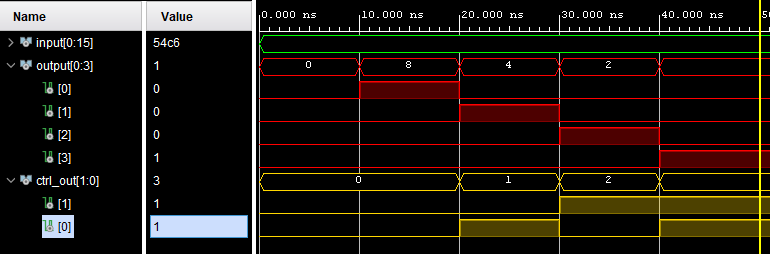
\includegraphics[width=0.9\linewidth]{figure/esercizio1-2/simulazione}
  \caption{Simulazione della rete di interconnessione 16:4}
  \label{fig:esercizio1-2:simulazione}
\end{figure}

L'ingresso \texttt{input[0:15]} vale 0x54C6 ($0101\,0100\,1100\,0110_2$) per tutta la durata mostrata, e il suo bit di indice 1 è \texttt{'1'}. Fino a \SI{10}{ns} le selezioni sono nulle: viene propagato \texttt{input(0)}, pari a \texttt{'0'}, e \texttt{output[0:3]} vale 0x0. A \SI{10}{ns} \texttt{ctrl\_in} diventa $0001_2$, quindi il multiplexer seleziona \texttt{input(1)}. Con \texttt{ctrl\_out} pari a $0_{10}$ l'uscita è 0x8 ($1000_2$), ossia \texttt{output(0)} a \texttt{'1'}; con $1_{10}$ è 0x4 ($0100_2$), con $2_{10}$ è 0x2 ($0010_2$) e con $3_{10}$ è 0x1 ($0001_2$). In ogni intervallo di \SI{10}{ns} è quindi attivo il solo bit selezionato, come richiesto dagli \texttt{assert} del testbench.
